%----------------------------------------------------------------------------------------
%    PACKAGES AND THEMES
%----------------------------------------------------------------------------------------

\documentclass[aspectratio=169,xcolor=dvipsnames]{beamer}
\usetheme{SimplePlus}

\usepackage{hyperref}
\usepackage{graphicx} % Allows including images
\usepackage{booktabs} % Allows the use of \toprule, |rule and \bottomrule in tables

%----------------------------------------------------------------------------------------
%    TITLE PAGE
%----------------------------------------------------------------------------------------

\title{Mathematical Foundations \\ of Reinforcement Learning}
\subtitle{Chapter 2: State Values and Bellman Equation}

\author{Minseok Seo}

\institute
{
    Artificial Intelligence Graduate School \\
    Gwangju Institute of Science and Technology (GIST) % Your institution for the title page
}
\date{\today} % Date, can be changed to a custom date

%----------------------------------------------------------------------------------------
%    PRESENTATION SLIDES
%----------------------------------------------------------------------------------------

\begin{document}

\begin{frame}
    % Print the title page as the first slide
    \titlepage
\end{frame}

\begin{frame}{Overview}
    % Throughout your presentation, if you choose to use \section{} and \subsection{} commands, these will automatically be printed on this slide as an overview of your presentation
    \tableofcontents
\end{frame}

%------------------------------------------------
\section{Motivating example 1: Why are returns important?}
%------------------------------------------------

\begin{frame}{Motivating example 1: Why are returns important?}
    
\begin{figure}
	\centering
	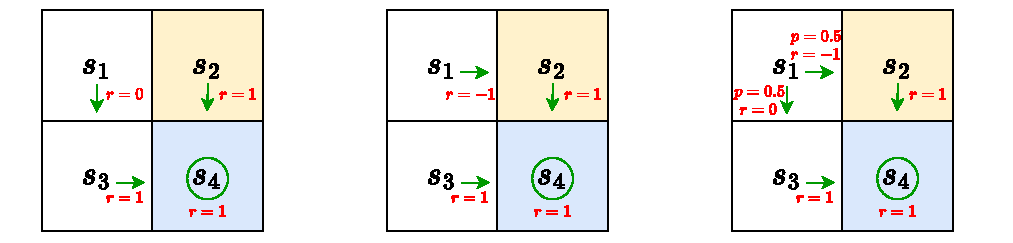
\includegraphics[width=0.7\textwidth]{../imgs/chap2/ex_importance_returns.pdf}
	\caption{Examples for demonstrating the importance of returns.}
	\label{fig:importance_returns}
\end{figure}

\begin{itemize}
	\item Following the first policy, discounted return is
	\begin{equation*}
		\begin{aligned}
			R_1 
			&= 0 + \gamma 1 + \gamma^2 1 + \cdots \\
			&= \gamma (1 + \gamma + \gamma^2 + \cdots) \\
			&= \frac{\gamma}{1 - \gamma} \\
		\end{aligned}
	\end{equation*}
	where $\gamma \in (0, 1)$ is the discount rate.
\end{itemize}

\end{frame}

%------------------------------------------------

\begin{frame}{Motivating example 1: Why are returns important?}
    
\begin{figure}
	\centering
	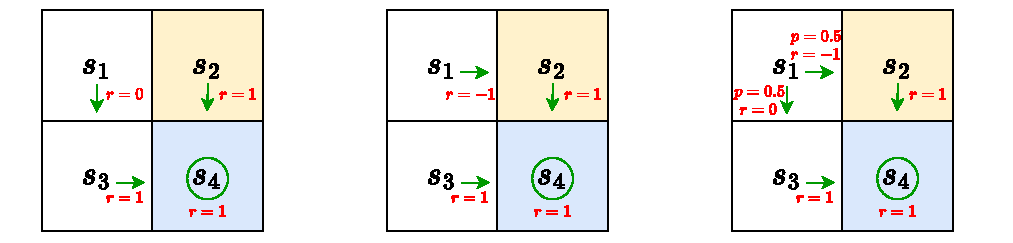
\includegraphics[width=0.7\textwidth]{../imgs/chap2/ex_importance_returns.pdf}
	\caption{Examples for demonstrating the importance of returns.}
\end{figure}

\begin{itemize}
	\item Following the second policy, discounted return is
	\begin{equation*}
		\begin{aligned}
			R_2 
			&= -1 + \gamma 1 + \gamma^2 1 + \cdots \\
			&= -1 + \gamma (1 + \gamma + \gamma^2 + \cdots) \\
			&= -1 + \frac{\gamma}{1 - \gamma} \\
		\end{aligned}
	\end{equation*}
\end{itemize}

\end{frame}

%------------------------------------------------

\begin{frame}{Motivating example 1: Why are returns important?}
    
\begin{figure}
	\centering
	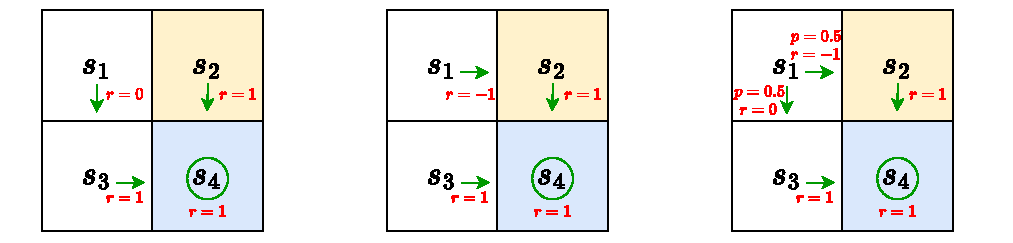
\includegraphics[width=0.7\textwidth]{../imgs/chap2/ex_importance_returns.pdf}
	\caption{Examples for demonstrating the importance of returns.}
\end{figure}

\begin{itemize}
	\item Following the third policy, discounted return is
	\begin{equation*}
		\begin{aligned}
			R_3
			&= 0.5 \left(-1 + \frac{\gamma}{1 - \gamma}  \right) + 0.5 \left(\frac{\gamma}{1 - \gamma} \right) \\
			&= -0.5 + \frac{\gamma}{1 - \gamma} \\
		\end{aligned}
	\end{equation*}
\end{itemize}

By Comparing the returns of the three policies, we notice that $R_1 > R_2 > R_3$ for any $\gamma$. \\
It is notable that $R_3$ does not strictly comply with the definition of returns because it is more like an expected value.

\end{frame}

%------------------------------------------------
\section{Motivating example 2: How to calculate returns?}
%------------------------------------------------

\begin{frame}{How to calculate returns?}

\begin{figure}
	\centering
	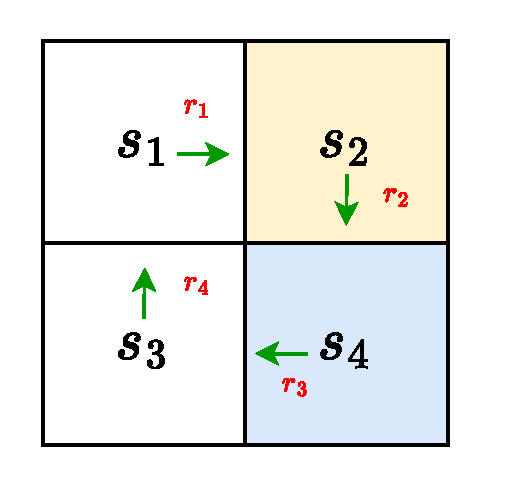
\includegraphics[width=0.2\textwidth]{../imgs/chap2/ex_calculate_returns.pdf}
	\caption{An example for demonstrating how to calculate returns.}
	\label{fig:calculate_returns}
\end{figure}

There are two ways to calculate returns: The first is simply by definition: a return equals the discounted sum of all rewards collected along a trajectory.
\begin{equation*}
	\begin{aligned}
		v_1 &= r_1 + \gamma r_2 + \gamma^2 r_3 + \cdots \\
		v_2 &= r_2 + \gamma r_3 + \gamma^2 r_4 + \cdots \\
		v_3 &= r_3 + \gamma r_4 + \gamma^2 r_1 + \cdots \\
		v_4 &= r_4 + \gamma r_1 + \gamma^2 r_2 + \cdots \\
	\end{aligned}
\end{equation*}

\end{frame}

%------------------------------------------------

\begin{frame}{How to calculate returns?}

\begin{figure}
	\centering
	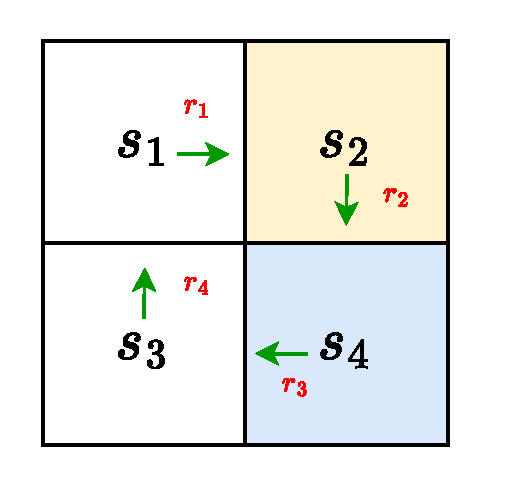
\includegraphics[width=0.2\textwidth]{../imgs/chap2/ex_calculate_returns.pdf}
	\caption{An example for demonstrating how to calculate returns.}
\end{figure}

The second way is based on the idea of bootstrapping.
\begin{equation} \label{eq:bootstrapping}
	\begin{aligned}
		v_1 &= r_1 + \gamma(r_2 + \gamma r_3 + \cdots) = r_1 + \gamma v_2 \\
		v_2 &= r_2 + \gamma(r_3 + \gamma r_4 + \cdots) = r_2 + \gamma v_3 \\
		v_3 &= r_3 + \gamma(r_4 + \gamma r_1 + \cdots) = r_3 + \gamma v_4 \\
		v_4 &= r_4 + \gamma(r_1 + \gamma r_2 + \cdots) = r_4 + \gamma v_1 \\
	\end{aligned}
\end{equation}

\end{frame}

%------------------------------------------------
\begin{frame}{How to calculate returns?}

The equation \ref{eq:bootstrapping} can be reformed into a linear matrix-vector equation:

\begin{equation} \label{eq:bootstrapping_matrix}
\underbrace{
\begin{bmatrix}
v_1 \\
v_2 \\
v_3 \\
v_4
\end{bmatrix}
}_{v}
=
\begin{bmatrix}
r_1 \\
r_2 \\
r_3 \\
r_4
\end{bmatrix}
+
\begin{bmatrix}
\gamma v_2 \\
\gamma v_3 \\
\gamma v_4 \\
\gamma v_1
\end{bmatrix}
=
\underbrace{
\begin{bmatrix}
r_1 \\
r_2 \\
r_3 \\
r_4
\end{bmatrix}
}_{r}
+
\gamma
\underbrace{
\begin{bmatrix}
0 & 1 & 0 & 0 \\
0 & 0 & 1 & 0 \\
0 & 0 & 0 & 1 \\
1 & 0 & 0 & 0
\end{bmatrix}
}_{P}
\underbrace{
\begin{bmatrix}
v_1 \\
v_2 \\
v_3 \\
v_4
\end{bmatrix}
}_{v},
\end{equation}

which can be written compactly as
\begin{equation*}
	v = r + \gamma P v.
\end{equation*}

\end{frame}

%------------------------------------------------
\section{State values}
%------------------------------------------------

\begin{frame}{State values}

Starting from $t$, we can obtain a state-action-reward trajectory:
\begin{equation*}
	S_t \xrightarrow{A_t} S_{t + 1}, R_{t + 1} \xrightarrow{A_{t + 1}} S_{t + 2}, R_{t + 2} \xrightarrow{A_{t + 2}} S_{t + 3}, R_{t + 3}  \xrightarrow{A_{t + 3}} \cdots
\end{equation*}

By definition, the discounted return along the trajectory is 
\begin{equation*}
	G_t = R_{t + 1} + \gamma R_{t + 2} + \gamma^2 R_{t + 3} + \cdots
\end{equation*}
where $\gamma \in (0, 1)$ is the discount rate.

\end{frame}

%------------------------------------------------

\begin{frame}{State values}

Note that $G_t$ is a random variable since $R_{t + 1}, R_{t + 2}, \cdots$ are all random variables. \\
Since $G_t$ is a random variable, we can calculate its expected value (also called the expectation or mean):
\begin{equation*}
	v_\pi(s) = \mathbb{E}[G_t | S_t = s]
\end{equation*}

\end{frame}

%------------------------------------------------
\section{Bellman equation}
%------------------------------------------------

\begin{frame}{Bellman equation}

We can be rewritten the $G_t$ as follows:
\begin{equation*}
	\begin{aligned}
		G_t
		&= R_{t + 1} + \gamma R_{t + 2} + \gamma^2 R_{t + 3} + \cdots \\
		&= R_{t + 1} + \gamma (R_{t + 2} + \gamma R_{t + 3} + \cdots) \\
		&= R_{t + 1} + \gamma G_{t + 1}
	\end{aligned}
\end{equation*}
where $G_{t + 1} = R_{t + 2} + \gamma R_{t + 3} + \cdots$. \\
This equation establishes the relationship between $G_t$ and $G_{t + 1}$.

\end{frame}

%------------------------------------------------
\begin{frame}{Bellman equation}


Then, the state value can written as
\begin{equation} \label{eq:state_value}
	\begin{aligned}
		v_\pi(s)
		&= \mathbb{E}[G_t | S_t = s] \\
		&= \mathbb{E}[R_{t + 1} + \gamma G_{t + 1} | S_t = s] \\
		&= \mathbb{E}[R_{t + 1} | S_t = s] + \gamma \mathbb{E}[G_{t + 1} | S_t = s] \\
	\end{aligned}
\end{equation}
The two terms in Eq. \ref{eq:state_value} are analzed next slide.

\end{frame}

%------------------------------------------------
\begin{frame}{Bellman equation}

The first term $\mathbb{E}[R_{t + 1} | S_t = s]$, is the expectation of the immediate rewards. \\
It can be calculated as follows:
\begin{equation} \label{eq:immediate_rewards}
	\begin{aligned}
		\mathbb{E}[R_{t + 1} | S_t = s]
		&= \sum_{a \in \mathcal{A}} \pi(a|s) \mathbb{E}[R_{t + 1} | S_t = s, A_t = a] \\
		&= \sum_{a \in \mathcal{A}} \pi(a|s) \sum_{r \in \mathcal{R}} p(r|s, a) r
	\end{aligned}
\end{equation}

\end{frame}

%------------------------------------------------
\begin{frame}{Bellman equation}


The second term $\mathbb{E}[G_{t + 1} | S_t = s]$, is the expectation of the future rewards. \\
It can be calculated as follows:
\begin{equation} \label{eq:future_rewards}
	\begin{aligned}
		\mathbb{E}[G_{t + 1} | S_t = s]
		&= \sum_{s \in \mathcal{S}} \mathbb{E}[G_{t + 1} | S_t = s, S_{t + 1} = s'] p(s'|s) \\
		&= \sum_{s' \in \mathcal{S}} \mathbb{E}[G_{t + 1} | S_{t + 1} = s'] p(s'|s) \quad \text{(due to the Markov property)} \\
		&= \sum_{s' \in \mathcal{S}} v_\pi(s') p(s'|s) \\
		&= \sum_{s' \in \mathcal{S}} v_\pi(s') \sum_{a \in \mathcal{A}} p(s'|s, a) \pi(a|s) \\
	\end{aligned}
\end{equation}

\end{frame}

%------------------------------------------------

\begin{frame}{Bellman equation}

Substituting Eq. \ref{eq:immediate_rewards} and Eq. \ref{eq:future_rewards} into Eq. \ref{eq:state_value}, we obtain the Bellman equation:
\begin{equation} \label{eq:bellman_equation}
	\begin{aligned}
		v_{\pi}(s) 
		&= \mathbb{E}[R_{t + 1} | S_t = s] + \gamma \mathbb{E}[G_{t + 1} | S_t = s], \\
		&= \underbrace{
				\sum_{a \in \mathcal{A}} \pi(a | s)
				\sum_{r \in \mathcal{R}} p(r | s, a) r
			}_{\text{mean of immediate rewards}}
			+ \underbrace{
				\gamma \sum_{a \in \mathcal{A}} \pi(a | s) 
				\sum_{s' \in \mathcal{S}} p(s' | s, a) v_{\pi}(s')
			}_{\text{mean of future rewards}} \\
		&= \sum_{a \in \mathcal{A}} \pi(a | s)
		\left[
			\sum_{r \in \mathcal{R}} p(r | s, a) r +
			\gamma \sum_{s' \in \mathcal{S}} p(s' | s, a) v_{\pi}(s')
		\right],
		\quad \text{for all } s \in \mathcal{S}.
	\end{aligned}
\end{equation}
This equation is in an elementwise form. \\
Since it is valid for every state, we can combine all these equations and write them concisely in a matrix-vector form.

\end{frame}

%------------------------------------------------
\section{Matrix-vector form of the Bellman equation}
%------------------------------------------------

%------------------------------------------------

\begin{frame}{Matrix-vector form of the Bellman equation}

\begin{equation} \label{eq:bellman_equation_matrix}
	\begin{aligned}
		v_{\pi}(s) 
		&= \mathbb{E}[R_{t + 1} | S_t = s] + \gamma \mathbb{E}[G_{t + 1} | S_t = s], \\
		&= \underbrace{
				\sum_{a \in \mathcal{A}} \pi(a | s)
				\sum_{r \in \mathcal{R}} p(r | s, a) r
			}_{r_\pi(s)}
			+ \gamma \sum_{s' \in \mathcal{S}} v_\pi(s')
			\underbrace{ 
				\sum_{a \in \mathcal{A}} p(s'|s, a) \pi(a|s)
			}_{p_\pi(s'|s)} \\
		&= r_\pi(s) + \gamma \sum_{s' \in \mathcal{S}} p_\pi(s'|s) v_\pi(s')
	\end{aligned}
\end{equation}
Here, $r_\pi(s)$ denotes the mean of the immediate rewards, and $p_\pi(s'|s)$ is the probability of transitioning from $s$ to $s'$ under policy $\pi$.

\end{frame}

\begin{frame}{Matrix-vector form of the Bellman equation}

Let $v_\pi = [v_\pi(s_1), v_\pi(s_2), \cdots, v_\pi(s_n)]^T \in \mathbb{R}^n, r_\pi = [r_\pi(s_1), r_\pi(s_2), \cdots, r_\pi(s_n)]^T \in \mathbb{R}^n$, and $P_\pi \in \mathbb{R}^{n \times n}$ with $[P_\pi]_{ij} = p_\pi(s_j|s_i)$. \\
Then, the Bellman equation can be written in a matrix-vector form:
\begin{equation} \label{eq:bellman_matrix_vector}
	v_\pi = r_\pi + \gamma P_\pi v_\pi.
\end{equation}
where $v_\pi$ is the unknown to be solved, and $r_\pi, P_\pi$ are known.

\begin{equation*}
	\underbrace{
	\begin{bmatrix}
	v_{\pi}(s_1) \\
	v_{\pi}(s_2) \\
	v_{\pi}(s_3) \\
	v_{\pi}(s_4)
	\end{bmatrix}
	}_{v_{\pi}}
	=
	\underbrace{
	\begin{bmatrix}
	r_{\pi}(s_1) \\
	r_{\pi}(s_2) \\
	r_{\pi}(s_3) \\
	r_{\pi}(s_4)
	\end{bmatrix}
	}_{r_{\pi}}
	+
	\gamma
	\underbrace{
	\begin{bmatrix}
	p_{\pi}(s_1|s_1) & p_{\pi}(s_2|s_1) & p_{\pi}(s_3|s_1) & p_{\pi}(s_4|s_1) \\
	p_{\pi}(s_1|s_2) & p_{\pi}(s_2|s_2) & p_{\pi}(s_3|s_2) & p_{\pi}(s_4|s_2) \\
	p_{\pi}(s_1|s_3) & p_{\pi}(s_2|s_3) & p_{\pi}(s_3|s_3) & p_{\pi}(s_4|s_3) \\
	p_{\pi}(s_1|s_4) & p_{\pi}(s_2|s_4) & p_{\pi}(s_3|s_4) & p_{\pi}(s_4|s_4)
	\end{bmatrix}
	}_{P_{\pi}}
	\underbrace{
	\begin{bmatrix}
	v_{\pi}(s_1) \\
	v_{\pi}(s_2) \\
	v_{\pi}(s_3) \\
	v_{\pi}(s_4)
	\end{bmatrix}
	}_{v_{\pi}}.
\end{equation*}

\end{frame}

%------------------------------------------------
\section{Solving state values from the Bellman equation}
%------------------------------------------------

\begin{frame}{Closed-from solution}

Since $v_\pi = r_\pi + \gamma P_\pi v_\pi$ is a simple linear equation, its closed-form solution can be easily obtained as follows:
\begin{equation*}
	v_\pi = (I - \gamma P_\pi)^{-1} r_\pi
\end{equation*}

\end{frame}

%------------------------------------------------
\begin{frame}{Iterative solution}

Although the closed-form solution is useful for theoretical analysis purposes, it is not applicable in practice because it involves a matrix inversion operation, which still needs to be calculated by other numerical algorithms. \\
In fact, we can directly solve the Bellman equation using the following iterative algorithm:
\begin{equation*}
	v_{k + 1} = r_\pi + \gamma P_\pi v_k, \quad k = 0, 1, 2, \cdots
\end{equation*}

This algorithm generates a sequence of vectors $\{ v_0, v_1, v_2, \cdots \}$, where $v_0 \in \mathbb{R}^n$ is an initial guess of $v_\pi$. \\
It holds that
\begin{equation*}
	v_k \rightarrow v_\pi = (I - \gamma P_\pi)^{-1} r_\pi, \quad \text{as } k \rightarrow \infty
\end{equation*}

\end{frame}

%------------------------------------------------
\section{Action values}
%------------------------------------------------

\begin{frame}{Action values}

The action value indicates the value of taking an action at a state.
\begin{equation*}
	q_\pi(s, a) = \mathbb{E}[G_t | S_t = s, A_t = a]
\end{equation*}
What is the relationship between action values and state values?

\end{frame}

%------------------------------------------------
\begin{frame}{From action value to state value}

First, it follows from the properties of conditional expectation that
\begin{equation*}
	\underbrace{\mathbb{E}[G_t | S_t = s]}_{v_{\pi}(s)}
	=
	\sum_{a \in \mathcal{A}}
	\underbrace{\mathbb{E}[G_t | S_t = s, A_t = a]}_{q_{\pi}(s, a)}
	\pi(a | s)
\end{equation*}
It then follows that
\begin{equation} \label{eq:action_value_state_value}
	v_{\pi}(s) = \sum_{a \in \mathcal{A}} \pi(a|s) q_{\pi}(s, a)
\end{equation}
Eq. \ref{eq:action_value_state_value} shows how to obtain state values from action values.

\end{frame}

%------------------------------------------------
\begin{frame}{From state value to action value}

Second, since the state value is given by Eq. \ref{eq:bellman_equation}
\begin{equation*}
	v_\pi(s) = \sum_{a \in \mathcal{A}} \pi(a | s)
	\underbrace{\left[ \sum_{r \in \mathcal{R}} p(r|s, a) r + \gamma \sum_{s' \in \mathcal{S}} p(s'|s, a) v_{\pi}(s') \right]}_{q_\pi(s, a)}
\end{equation*}
comparing it with Eq. \ref{eq:action_value_state_value}, leads to:
\begin{equation} \label{eq:state_value_action_value}
	q_\pi(s, a) = \sum_{r \in \mathcal{R}} p(r|s, a) r + \gamma \sum_{s' \in \mathcal{S}} p(s'|s, a) v_{\pi}(s')
\end{equation}
Above Eq. \ref{eq:state_value_action_value} shows how to obtain action values from state values.

\end{frame}

%------------------------------------------------
\begin{frame}{The Bellman equation in terms of action values}

Substituting Eq. \ref{eq:action_value_state_value} into Eq. \ref{eq:state_value_action_value}, we can rewrite the Bellman equation in terms of action values:
\begin{equation*}
	q_\pi(s, a) = \sum_{r \in \mathcal{R}} p(r|s, a) r + \gamma \sum_{s' \in \mathcal{S}} p(s'|s, a) \sum_{a' \in \mathcal{A}(s')} \pi(a'|s') q_\pi(s', a')
\end{equation*}

\end{frame}

%----------------------------------------------------------------------------------------

\end{document}